\documentclass[utf8,xcolor=table]{beamer}

\usepackage[T2A]{fontenc}
\usepackage[utf8]{inputenc}
\usepackage[english,russian]{babel}
%\usepackage{tikz-uml}
\usepackage{minted}
\usepackage{cmap}

\hypersetup{colorlinks,linkcolor=blue,urlcolor=blue}

\mode<presentation>{
	\usetheme{CambridgeUS}
}

\renewcommand{\t}[1]{\ifmmode{\mathtt{#1}}\else{\texttt{#1}}\fi}
\newcommand{\svgimg}[1]{
  \begin{center}
	\includegraphics[scale=1]{#1.pdf}
  \end{center}
}

\title[ООП]{Объектно-ориентированное программирование}
\author{Егор Суворов}
\institute[НИУ ВШЭ]{Курс <<Основы программирования>>}
\date[21.11.2019]{Четверг, 21 ноября 2019 года}

\setlength{\arrayrulewidth}{1pt}

\begin{document}

\begin{frame}
\titlepage
\end{frame}

% !TeX root = 191121.tex
\begin{frame}[t]{Базовый синтаксис классов и объектов}
Класс "--- структура с методами, добавляет удобный синтаксис?

Демо!
\end{frame}

\begin{frame}[t]{Тонкости Python}
\begin{itemize}
\item Класс "--- это лишь каркас для объектов.
\item У почти любого объекта можно добавлять-удалять поля.
\item Как хранится в памяти "--- неважно и не знаем.
\item \texttt{self} передаётся как явный параметр.
\item Нет приватных методов и полей, только договорённости.
\end{itemize}
\end{frame}

\begin{frame}[t,fragile]{Зачем ещё объекты?}
\begin{itemize}
\item Хотим улучшить \textit{композируемость} кусочков программы.
\item Процедура может только вызвать другую процедуру с параметрами.
\item Если хотим изменить, кого вызвать "--- надо явно передавать все параметры и действия:
\begin{minted}{cpp}
void apply(
    intrusive_list *list,
    void (*op)(intrusive_node *node, void *data),
    void *data
);
int mergesort(
    void *array,
    size_t elements, size_t element_size,
    int (*comparator)(const void*, const void*)
);
\end{minted}
\end{itemize}
\end{frame}

\begin{frame}[t]{Всё есть объект}
Объект "--- кусок программы со своим состоянием и методами.

Тогда становится сильно меньше примитивов:
\begin{itemize}
	\item Примитив данных "--- объект.
	\item Примитив кода "--- вызов метода.
\end{itemize}

Демо!
\end{frame}

\begin{frame}[t]{Определения}
Определения работают и для ООП, и для модулей, и для функций.

\begin{itemize}
\item
	\textit{Контракт}/\textit{интерфейс} "--- соглашение о том, как
	и когда можно вызывать методы объекта (или процедуры), что возвращают.
\item
	\textit{Инвариант} "--- соглашении о внутреннем состоянии объекта
	(или цикла), внешний мир о нём не знает.
\item
	\textit{Интерфейс} "--- технический способ описать кусок контракта
	отдельно от реализации: какие функции с какими именами требуются.
	Есть в Java.
	В C++ и Python являются частным случаем \textit{абстрактных базовых классов}.
\item
	\textit{Инкапсуляция} "--- идея о том, что детали реализации объекта
	(функции, модуля) внешний мир видеть не должнен и не должен от них
	зависеть.
	Хорошо сочетается с интерфейсами и статической типизацией:
	просто нельзя вызвать метод, не описанный в интерфейсе, даже если он есть.
\end{itemize}
\end{frame}

\begin{frame}[t]{Исключения}
Способ обработки ошибок:
\begin{itemize}
\item Исключение \textit{выбрасывается}/\textit{поднимается}.
\item Все функцию делают как-бы-\texttt{return}, пока не найдётся кто-то,
	кто \textit{знает}, что делать с ошибкой.
\item Если никто не знает "--- программа завершается.
\end{itemize}

Демо!
\end{frame}

\begin{frame}[t]{Исключения "--- важное}
\begin{itemize}
\item Ловите \textit{только} те исключения, про которые точно знаете,
	от чего они возникают и что с ними делать.
\item Исключение из правила: хотим попробовать изолировать друг от друга
	кусочки системы.
	Тогда может вылететь любое исключение "--- это полный сбой подсистемы,
	надо что-то делать.
\item Не игнорируйте исключения.
\end{itemize}
\end{frame}

\begin{frame}[t]{Параметрический полиморфизм}
\begin{itemize}
\item
	Можем написать код один раз, а он работает с объектами разных типов.
\item
	В Python "--- \textit{утиная типизация}: для работы с объектом требуется
	лишь наличие методов с нужными именами и их ожидаемое поведение.
\item
    \textbf{Если оно выглядит как утка, плавает как утка и крякает как утка, то это, вероятно, и есть утка.}
\item
	В Java/C++ требуется явно указать, что объект реализует некий \textit{интерфейс},
	тогда компилятор статически проверит и код, и тех, кто его вызывает.
\item
	В Python, впрочем, тоже можно статически проверить (появляются \textit{подтипы}).
\item
	В C++ есть шаблоны, там утиная типизация.
\item
	В Haskell "--- как в Java, только компилятор может сам догадаться о требованиях.
\end{itemize}
\end{frame}

% !TeX root = 191121.tex
\begin{frame}[t]{Домашнее задание: задача}
Как удобно писать Telegram-ботов?

Требования:
\begin{itemize}
\item Можно писать бота и не думать о Telegram Bot API.
\item Можно тестировать автоматически.
\item Можно тестировать бота отдельно от логики игры.
\end{itemize}
\end{frame}

\begin{frame}[t]{Архитектура-1}
\begin{center}
	\includegraphics[width=\textwidth]{general-bot-arch.pdf}
\end{center}
\end{frame}

\begin{frame}[t]{Связность и зацепление}
\begin{center}
	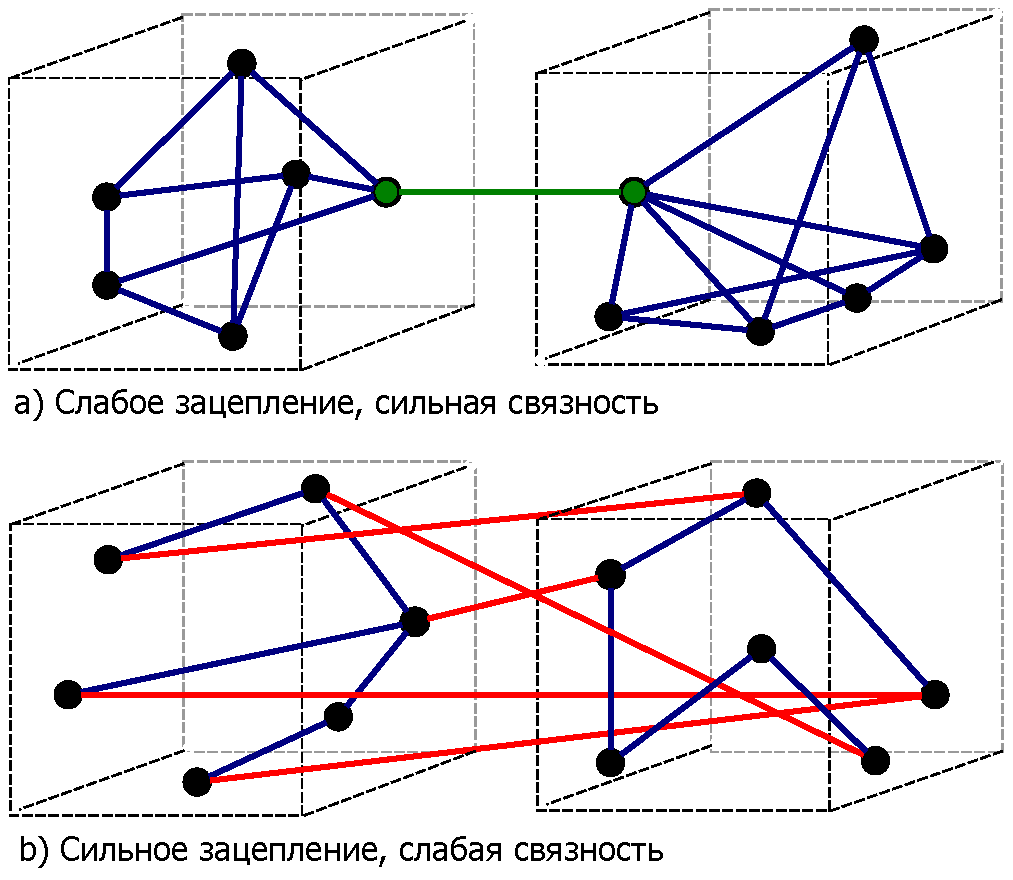
\includegraphics[height=0.8\textheight]{CouplingVsCohesion.pdf}
\end{center}
\end{frame}

\begin{frame}[t]{Архитектура-2}
\begin{center}
	\includegraphics[width=\textwidth]{user-independent-bot-arch.pdf}
\end{center}
\end{frame}

\begin{frame}[t]{Чего добились}
\begin{itemize}
	\item Можно написать $N$ способов запуска бота и $M$ ботов за $\mathcal O(N+M)$ кода.
	\item В частности, один из способов запуска "--- автоматические тесты.
	\item Из-за \texttt{UserIndependentBot} в боте нельзя послать сообщение не тому пользователю.
	\item В процедурном стиле пришлось бы протаскивать много-много параметров.
\end{itemize}
\end{frame}


\end{document}
